%%%%%%%%%%%%%%%%%%%%%%%%%%%%%%%%%%%%%%%%%%%%%%%%%%%%%%%%%%%%%%%%%%%%%%%%%%%%%%%%
%2345678901234567890123456789012345678901234567890123456789012345678901234567890
%        1         2         3         4         5         6         7         8

\documentclass[letterpaper, 10 pt, conference]{ieeeconf}  % Comment this line out
                                                          % if you need a4paper
%\documentclass[a4paper, 10pt, conference]{ieeeconf}      % Use this line for a4
                                                          % paper

\IEEEoverridecommandlockouts                              % This command is only
                                                          % needed if you want to
                                                          % use the \thanks command
\overrideIEEEmargins
% See the \addtolength command later in the file to balance the column lengths
% on the last page of the document

\usepackage{graphicx}

% The following packages can be found on http:\\www.ctan.org
%\usepackage{graphics} % for pdf, bitmapped graphics files
%\usepackage{epsfig} % for postscript graphics files
%\usepackage{mathptmx} % assumes new font selection scheme installed
%\usepackage{times} % assumes new font selection scheme installed
%\usepackage{amsmath} % assumes amsmath package installed
%\usepackage{amssymb}  % assumes amsmath package installed

\title{\LARGE \bf
Parallelizing Logistic Regression
}

%\author{ \parbox{3 in}{\centering Huibert Kwakernaak*
%         \thanks{*Use the $\backslash$thanks command to put information here}\\
%         Faculty of Electrical Engineering, Mathematics and Computer Science\\
%         University of Twente\\
%         7500 AE Enschede, The Netherlands\\
%         {\tt\small h.kwakernaak@autsubmit.com}}
%         \hspace*{ 0.5 in}
%         \parbox{3 in}{ \centering Pradeep Misra**
%         \thanks{**The footnote marks may be inserted manually}\\
%        Department of Electrical Engineering \\
%         Wright State University\\
%         Dayton, OH 45435, USA\\
%         {\tt\small pmisra@cs.wright.edu}}
%}

\author{Wansang Lim$$ and Valerie Angulo$$% <-this % stops a space
%\thanks{*This work was not supported by any organization}% <-this % stops a space
%\thanks{$^{1}$H. Kwakernaak is with Faculty of Electrical Engineering, Mathematics and Computer Science,
%        University of Twente, 7500 AE Enschede, The Netherlands
%        {\tt\small h.kwakernaak at papercept.net}}%
%\thanks{$^{2}$P. Misra is with the Department of Electrical Engineering, Wright State University,
%        Dayton, OH 45435, USA
%        {\tt\small p.misra at ieee.org}}%
}


\begin{document}



\maketitle
\thispagestyle{empty}
\pagestyle{empty}


%%%%%%%%%%%%%%%%%%%%%%%%%%%%%%%%%%%%%%%%%%%%%%%%%%%%%%%%%%%%%%%%%%%%%%%%%%%%%%%%
\begin{abstract}
  Logistic regression is a statistical analysis tool used as a predictive analytic in a variety of disciplines. In this paper, we focus on parallelizing binary logistic regression analysis for predictive analytics in data science for environmental science datasets. Parallelizing logistic regression would improve computation time and decrease memory latency when analyzing large data sets, allowing for more data to be processed faster. In this paper, we compare a sequential implementation of binary logistic regression with a CUDA implementation, a parallelized R implementation and a multiprocessor OpenCV version, looking at the relationship between dataset sizes and time taken to process the data. Our findings point to improvements in computation time and less memory latency for CUDA versions of logistic regression.

\end{abstract}


%%%%%%%%%%%%%%%%%%%%%%%%%%%%%%%%%%%%%%%%%%%%%%%%%%%%%%%%%%%%%%%%%%%%%%%%%%%%%%%%
\section{INTRODUCTION}

Logistic Regression is used as a predictive analytic in many disciplines ranging from biology and conservation to business. It models a binary dependent and one or more binary or nonbinary independent variables. This is useful in cases of observing phenomena that may occur due to a specific event. The purpose of logistic regression is to predict the occurrence of phenomena based on acquired current data. Mathematically, the binary dependent variable is either 0 or 1 and indicates the presence or absence of a certain condition, such as alive/dead or win/lose, that may be related to the independent conditions. In this paper, we are primarily concerned with the applications of binary logistic regression analysis for predictive analytics in data science, particularly for environmental science datasets. For our purpose, logistic regression is used to classify dependent variables into different groups.

Currently, there is an abundance of large datasets that are open sourced and easily accessible to the public. This is especially beneficial for scientific research. However, processing large data sets is time consuming and resource intensive for CPU in terms of memory and computation time. Sequential implementations of logistic regression require a lot of time to process smaller amounts of data and have a high memory latency. Implementation of a parallelized binary logistic regression would allow for an increased amount of data to be processed in less time and with less resource intensive computations. Logistic regression is an excellent analytic to parallelize because it primarily utilizes matrix multiplication, which is easy to convert to parallel code. It also utilizes an inverse function which is a variation of matrix multiplication and determines the natural log of a matrix, a function that is easily supported by parallelism. In this paper, we compare a sequential implementation of binary logistic regression with a CUDA implementation, a parallelized R implementation and a multiprocessor OpenML(???) version, looking at the relationship between dataset sizes and time taken to process the data. Our findings point to improvements in computation time and less memory latency for CUDA versions of logistic regression, as well as parallelized R implementations.


\section{BACKGROUND}

Logistic regression is a predictive analytic that is used to categorize data into different groups. It can be binomial, ordinal or multinomial and is based on linear regression; a logistic regression estimates a multiple linear regression function. It is the correct regression to use if there is a binary dependent variable, such as time spent studying versus whether a student passes or fails a course, or other situations depending on independent variables such as win/lose, dead/alive, yes/no, present/absent etc. Binary logistic regression is used to describe the relationship between a binary dependent variable and one or many independent variables. This predictive analytic tool is useful in data science and many other fields for predicting how likely an event will occur when certain independent factors are present. Following are the steps needed to implement a logistic regression.

\subsection{Linear Regression}
In order to do a logistic regression, we must first start with a linear regression.

$$Y = b_0 + b_1X_1 + b_2X_2 + b_nX_n$$

In this linear model, the x’s are the predictors/independent variables and the Bn’s are the parameters of the model or the coefficients of the independent variables, with $b_0$ being a constant term. The Y value is the outcome /dependent variable and can vary from negative to positive infinity for a linear regression.  %The graph for a linear regression is shown below, note how it can extend infinitely in both directions: (insert graph)

\subsection{Logistic Function}
The next step is to turn the linear regression into a sigmoid function, also known as a logistic function. 

$$p(x) =  \frac{1}{1+e^{-x}}   =   \frac{e^x}{1+e^x} 
= \frac{e^{(b_0 + b_1X_1 + ... + b_nX_n)}}{1+e^{(b_0 + b_1X_1 + ... + b_nX_n)}}$$

P(x) is the probability of the dependent variable equaling a success. E(Y) is the expected value of the binary dependent variable Y. X is the linear regression formula. The function is as such because the range of p(x) should be between 0 to 1, rather than -infinity to +infinity. This function provides a limited range of values for probability, so the odds of the probability must be taken next to fully convert this logistic function into a logistic regression. %The graph for a logistic function is shown below, note how it extends across the y-axis: (insert graph)

\subsection{Logistic Regression} 
The logistic regression is the natural log of the inverse of the logistic function. The core of logistic regression is estimating the log odds of an event, also known as the logit of the probability, where the log odds is a prediction of the odds of a dependent variable based on one or more binary or real valued independent predictors/x-values.

The odds are determined by the inverse of the logistic function, where the probability of an outcome’s success (Y) is divided by the probability that it will not occur (1-Y). To determine the log-odds of an event occurring, we must take the natural log of this inverse. The purpose of this is to fit the logit of the probability of success with the predictors/x-values. We are then able to obtain a continuous predictor for the odds of an event happening.

$$logit p(x) = ln[\frac{p(x)}{1-p(x)}]$$

The dependent variable turns into a logit variable (the natural log of the odds of the dependent variable occurring or not). We then estimate the probability of the occurrence of a certain event based on the independent variables. The logit serves as a link between the linear regression and logistic function. The probability of success of obtaining a particular value from a binary dependent is equivalent to the odds of the dependent variable Y equaling a particular case.

$$ln[\frac{Y}{1-Y}] = b_0 + bX$$

Logistic regression seeks to find the equation that best predicts the value of Y for each value of X. The Y variable in logistic regression is the probability of obtaining a particular value of a binary variable, whereas the Y variable in linear regression is measured directly. %The graph for a logistic regression is shown below, note how the values are between 0 and 1 and are measured continuously: (insert graph)


\section{LITERATURE SURVEY}
We've looked at a variety of papers regarding parallelizing logistic regression, as well as the applications of parallelized and sequential logistic regressions. The following related works are presented because they either implement a biostatistic(?) model of logistic regression or they compare sequential and parallel versions of logistic regression. 

\subsection{Biostatistic Logistic Regression}
The algorithm that we have coded sequential and parallel versions of is applicable to biology and environmental studies. The work done by (Deforestation modelling using logistic regression and GIS) uses logistic regression in the manner that we implement and parallelize. In their work, they(NAMES!) look at binary logistic regression, determining whether deforestation is present or not in an area based on slope as an independent variable. The setup of the experiment is similar to ours, and their work is what drove us to parallelize logistic regression for scientific fields. While they analyze a sequential version of the logistic regression, there is no attempt to parallelize it. The data input is also far different than ours, where the focus is to use GIS with logistic regression, making comparison with their work difficult. They(NAMES!) analyze digital thematic-topographic maps with 63 different data layers such as forests, ranges and gardens. Our tests read data from a file containing random input values that fall within a certain range to represent our x and b values, rather than topographic maps or open source data.

\subsection{Parallelizing Logistic Regression}
Others, such as (NAMES liang, choi)(Evaluating Parallel Logistic Regression Models citation!), have parallelized the logistic regression for machine learning. Liang et. all(?) have looked at parallelized regressions in distributed platforms, parallel algorithms and sub-linear approximations. They worked with Hadoop and Spark, two distributed systems used in data science and analytics, to run sequential and parallel versions of code and compare platform/algorithm combinations with sub-linear algorithms specific to machine learning. This is clearly useful for machine learning but is not applicable to other fields that utilize logistic regression. Liang et all focus on parallelizing machine learning algorithms, while we are looking to parallelize logistic regression itself. They used five open datasets related to machine learning to make sure that they could accurately compare their methods whereas our data is randomly generated and doesn’t come from open source. Using open datasets are beneficial because the results allow for comparability with the performance of sequential machine learning algorithms that already exist. 

The work done by (NAMES) in (Breast Cancer Prediction by Logistic Regression with CUDA Parallel Programming Support)(CITE) focuses on parallelizing logistic regression for the purposes of machine learning, bioinformatics and data analysis. While it is primarily a machine learning approach and our work aims to be more generalized, the parallelization is reached by using CUDA parallel programming support, which we use in our experimental design as well. However, not much detail is gone into about how CUDA is implemented, only that different CUDA software versions are compared in determining the loss function for the machine learning logistic regression. Nevertheless, this work is useful in that it this approach is applicable to bioinformatics and data analysis. The dataset used is a real dataset containing anonymized patient information obtained from the Wisconsin Diagnostic Breast Cancer database. It contains 569 instances, with each instance corresponding to a patient (CITE!!!). This is beneficial in that the results obtained can be tested in real life, and they are. From the estimated Y values obtained per patient, there was a better chance at predicting whether a patient had breast cancer or not.  


\subsection{Implementations Used or Referenced} 
In Evaluating Parallel Logistic Regression Models (CITE), Liang and Choi implement a binary logistic regression, and we reference the parallel algorithm approach, but without the distributed platform or sub-linear approximation. They analyze their experimental results in accuracy, efficiency, scalability, robustness and running time. We analyze our results in terms of accuracy and running time and use this work as a reference on how to proceed with such an analysis. 

From (NAME et. all’s) work in Deforestation modelling using logistic regression and GIS, we use a similar logistic regression and proceed with the sequential code and then the parallelized code in a step-by-step approach as well. We break down our implementation into linear regression, then logistic function and finally into logistic regression in order to code logistic regression. (NAMES) use $R^2$ chi square test(?) to determine the fitness of their model, which is something we consider in our work but did not have enough time to do.


\section{PROPOSED SOLUTION}
We aim to parallelize the logistic regression as applied to biology and data science by using CUDA. There has been a lot of research on parallelizing logistic regression for machine learning techniques and algorithms, but nothing that we’ve seen that is general enough to cover parallelized logistic regression outside of machine learning purposes. The biostatistic research that we have come across uses sequential logistic regression with other new technologies but does not attempt to parallelize the logistic regression itself. From our research, we haven’t found others who attempt to parallelize a general logistic regression using CUDA. Therefore, we propose to parallelize the logistic regression in order to improve predictive behavior in a number of fields. The purpose of this is to show that logistic regression can be parallelized and used to analyze more data in less time.

\section{EXPERIMENTAL SETUP}

\subsection{Assumptions}
For our experiment we are implementing a binary logistic regression where our dependent variable is either 0 or 1 while our independent x variables are real numbers ranging from -3 to 3. To make sure our generated data set is valid, we followed the assumptions of data used for logistic regression applications. This involves having a binary dependent variable, not having outliers present in the data or strong correlations between independent data sets, and making sure no x values are below -3.29 or above 3.29. (https://www.statisticssolutions.com/what-is-logistic-regression/). Another consideration we took into account is the model fit. Having more independent x variables increases the amount of variance ($R^2$) but adding too many x variables will decrease the generalizability of the predictive analytic, thus decreasing its accuracy. During our analysis we made sure not to have a very large number of columns, which represents our x variables, so that we could model prime data sets used for logistic regression. To analyze the accuracy of our logistic regression, we computed its goodness-of-fit based on the Chi square test, as well as the amount of variance $R^2$. 

\subsection{Methods}
We decided to use a matrix of random values for our input data, where the user chooses the number of rows and columns. The rows represent the number of samples that data is acquired for while the columns within each row represent the number of independent x variables. For example, rows could represent a patient and the columns could represent independent factors that may determine whether the patient has a certain illness or not. We chose this presentation of data so that we could calculate matrix multiplication and inversion for sequential and CUDA code. 

To code our sequential version of a logistic regression, we broke down the logistic regression as described in the background section. An array of all the x values are read in from the file and transposed into a new array. X’ and X are then multiplied together (X’X). We then calculate the inverse of the transposed X which is (-1*X') and then we perform matrix multiplication on (X’X) and (-1*X’) . The value obtained is then multiplied with Y values to produce B values. From these B values that are produced, we populate an array of new X values and combine them with the B values to give us a predicted Y value. 

For our CUDA code, we used the same logic as the sequential code but we parallelized  matrix multiplication, inverse …etc…

\subsection{Machine Setup}

We used NYU linux CIMS accounts to run our sequential and parallelized logistic regression code. Before running the sequential and parallelized code, we made sure to generate the random data files that we needed to run our code with. To do this we compiled the random data program and then ran it with our specified number of rows and columns. From here, to run the parallelized code we used the cuda5 machine on the NYU prince cluster and loaded the cuda version 9.1 module. For the sequential code, we used the snappy machine on NYU’s prince cluster to obtain faster results for sequential code. We used the time flag to record time taken to compute the logistic regression of our sequential code and CUDA code, and we used nvprof to profile our CUDA code. 

\section{RESULTS AND DISCUSSION}

For our results, we used time to obtain the real time our programs took to compute the B values. We took an average of 5 time values per column per row to obtain a more accurate time.

\subsection{Sequential Results}
The results for our sequential code show a very small difference per change in row value (number of individuals). However, there is an increase in time with each increment of the column number, the number of independent variables, that appears to increase exponentially (Fig 1). Beyond column 12, we were unable to obtain results because time took longer than 1 hour, even when we use crunchy3 and snappy3 machines for quicker sequential computing. This limited our ability to properly compare our sequential results with our CUDA results. Differences in CUDA for column values as small as 2-12 did not provide much insight. We still obtained results for CUDA values that match sequential values. 

Figure 1 shows that the difference between row number is very small, but the difference between column numbers with a constant row number vary exponentially. In the table CITE/MAKE THIS TABLE!!! the differences of the time between columns for a constant row number are seen. Because the values of the columns varied greatly, but the values between rows stayed close, we decided not to test more rows out. The column numbers are the independent variables, the values along the x-axis of a matrix. Through our results, the more variables that are present per row, the exponentially greater time it takes to do matrix multiplication and inverse on the data matrix. We believe this is due to the recursion present in the sequential code, particularly in calculating the matrix inversion. We believe that there is little variation among row values because in calculating logistic regression multivariable logistic regression, the data samples/individuals/rows are averaged together to find a general Y value for all samples, but the inversions and high overhead operations are being performed on the independent variables, or column values. Therefore, sequential code is able to handle a large value of rows. 

We tested with row values of 10,000, 50,000 and 100,000 but received segmentation fault errors (TABLE X). However, a slow increase of time is noticed, where at row = 100,000 the time it takes to compute 2 variables per row increases by 10, compared to where row = 100. 

MAKE A TABLE EXACTLY LIKE SEQUENTIAL BUT FOR CUDA. MAKE A SCATTER with Rows = 20 and plot the columns, showing how it exponentially increases. the average of 5 times per column value. This can be a log graph????


\subsection{CUDA Results}

We checked if exponential performance difference depends on column number for our parallel code, as it does with our sequential code and found that the CUDA performance does not depend on column number up to 100 (Fig 2). So we focused on the number of rows for our CUDA code. Fig 2 shows that the column number of CUDA code up to 100 has no effect on performance. For our purposes, the number of independent variables, or column number in our project, is less than around 20 in papers for biology and environmental modeling.CITE THIS. Because of this, we checked the effect of sample numbers while the column number is limited to 20. In both column number 10 and 20, the performance of CUDA code is unstable up to 1000 and 2000. After that, the performance is almost proportional to sample or row numbers (Fig 3 and Fig 4).


\subsection{Comparing Both}

For the sequential code, at column 12, the time is around 400 seconds up to 1000 rows (Fig 1). We checked cuda performance for the same condition. The time for CUDA code with a row of 1000 dramatically reduced to 0.3 seconds, making it 1333 times faster than its other values(CUDA values or sequential values?). 

Currently, we are planning to compare algorithm for matrix inversion. For sequential code, we use adjoint and cofactor for matrix inversion. It has recursion which is not good for cuda code. We used Gaussian elimination to get matrix inversion. With this comparison, we can remove algorithm effect. Our row number limitation is about 100,000 ~ 20,000. We will try tiling for matrix multiplication to expand row numbers.  


\section{CONCLUSIONS}

Summary of what we found, why its useful, future implementations or things we'd do or change.

\begin{itemize}

\item recursive nature of logistic regression in sequential code greatly limits the time it takes to compute an increasing number of independent variables. 
\item CUDA code gracefully handles a large input of independent variables but could be improved in number of sample size.
\item In practical terms, biology and environmental science use around 20 independent variables at maximum.
\item We would like to improve our CUDA code to make it more efficient in processing a larger sample size, such as a size of 1,000,000 individuals or more.
\item We find that our CUDA code is adequate at processing large numbers of independent variables.
\item We would like to balance CUDA codes processing large amounts of independent variables for the ability to process very large sample sizes.
\end{itemize}


%%%%%%%%%%%%%%%%%%%%%%%%%%%%%%%%%%%%%%%%%%%%%%%% ALL OF OUR FIGURES AND TABLES

%\subsection{Figures and Tables}

Positioning Figures and Tables: Place figures and tables at the top and bottom of columns. Avoid placing them in the middle of columns. Large figures and tables may span across both columns. Figure captions should be below the figures; table heads should appear above the tables. Insert figures and tables after they are cited in the text. Use the abbreviation ÒFig. 1Ó, even at the beginning of a sentence.

\begin{table}[h]
\centering
\caption{Sequential code time results per row and column value. Time is in seconds, these results were obtained through snappy3 CIMS machine.}
\label{seq_ex}
\begin{center}
\begin{tabular}{|c|c|c|c|c|c|c|c|c|c|}
\hline
Col & Row = 16 & Row = 20 & Row = 50 & Row = 100 & Row = 500 & Row = 1000 & Row = 10000 & Row = 50000 & Row = 100000\\
\hline
2 & 0.0168 & 0.0104 & 0.0134 & 0.0116 & 0.0106 & 0.008 & 0.016 & 0.07 & 0.146 \\
\hline
4 & 0.016 & 0.01 & 0.0046 & 0.0112 & 0.0104 & 0.0082 & 0.025 & 0.112 & 0.228 \\
\hline
6 & 0.0148 & 0.0112 & 0.0062 & 0.0134 & 0.081 & 0.0096 & 0.034 & 0.157 & 0.31 \\
\hline
8 & 0.031 & 0.035 & 0.0276 & 0.0364 & 0.1254 & 0.032 & 0.066 & NAN & NAN \\
\hline
10 & 2.5764 & 2.602 & 2.615 & 2.5568 & 2.8394 & 2.5564 & NAN & NAN & NAN \\
\hline
12 & 397.905 & 395.137 & 396.281 & 396.541 & 395.702 & 395.609 & NAN & NAN & NAN \\
\hline
\end{tabular}
    %%  \caption{Inductance of oscillation winding on amorphous
    %%   magnetic core versus DC bias magnetic field}
    %\caption{Our Sequential Code}
\end{center}
\end{table}
%%%%%%%%%%%%%%%%%%%%%%%%%%%%%%%%%%%%%%%%%%%%%%%%%

   \begin{figure}[thpb]
      \centering
     % \framebox{\parbox{3in} {We suggest that you use a text box to insert a graphic (which is ideally a 300 dpi TIFF or EPS file, with all fonts embedded) because, in an document, this method is somewhat more stable than directly inserting a picture.
	 %}}
  		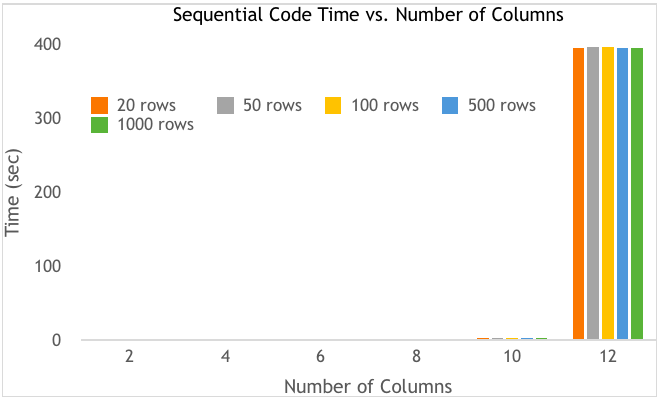
\includegraphics[width=\linewidth]{seqcode2.png}
  		%\caption{Our Sequential Code}
  		\label{fig:seq1}
  		\caption{Sequential code performance for logistic regression with varying number of columns and rows. Each bar represents a different value for the row input, and all row values obtained are compared with column time values.}
  	%}
   \end{figure}

	\begin{figure}[thpb]
		\centering
		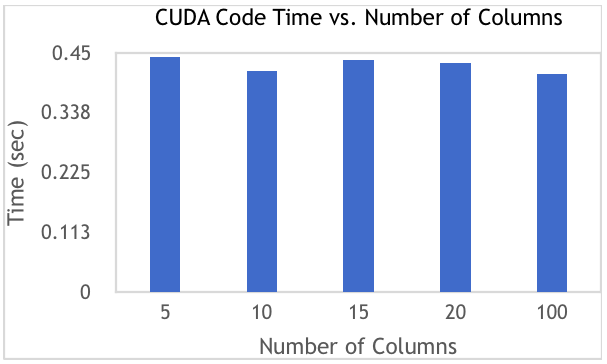
\includegraphics[width=\linewidth]{cudacolumns.png}
		%\caption{Our CUDA Code}
		%\label{fig:seq1}

		\caption{Performance difference of CUDA code between column number (5~20). The row number is set to 20 for all column numbers except for column = 100. The row number = 100 for column = 100.}
	\end{figure}

	\begin{figure}[thpb]
		\centering
		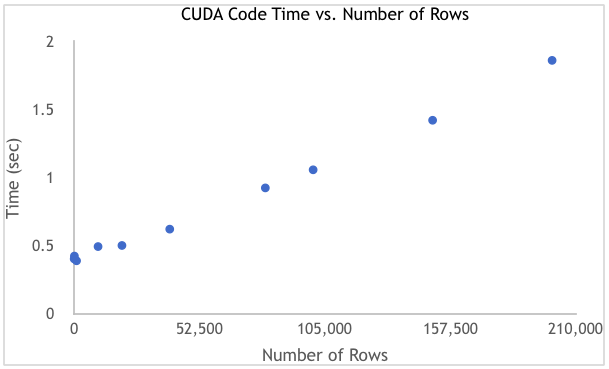
\includegraphics[width=\linewidth]{cudarow10.png}
		%\caption{Our CUDA Code}
		%\label{fig:seq1}
		\caption{Performance difference of CUDA code with a constant column value of 10.}
	\end{figure}

	\begin{figure}[thpb]
		\centering
		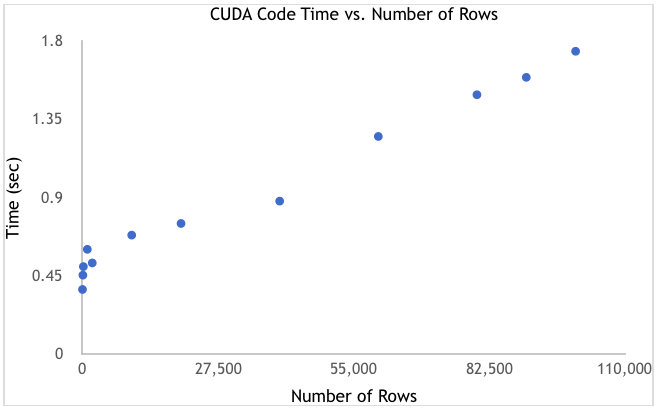
\includegraphics[width=\linewidth]{cudarow20.png}
		%\caption{Our CUDA Code}
		%\label{fig:seq1}
		\caption{Performance difference of CUDA code with a constant column value of 20.}
	\end{figure}	

%   \begin{figure}
%   		\centering
%  		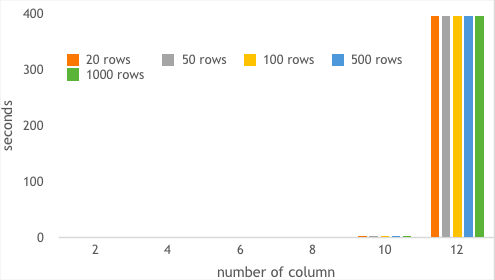
\includegraphics[width=\linewidth]{sequentialcode.png}
%  		\caption{Our Sequential Code}
%  		\label{fig:seq1}
%	\end{figure}

%Figure \ref{fig:seq1} shows a boat.

%%%%%%%%%%%%%%%%%%%%%%%%%%%%%%%%%%%%%%%%%%%%%%%%%%%%%%%%%%%%%%%%%%%%%%%%%%%%%%%%%%%%%%%%%%%%%%%%%%%%%%

\addtolength{\textheight}{-12cm}   % This command serves to balance the column lengths
                                  % on the last page of the document manually. It shortens
                                  % the textheight of the last page by a suitable amount.
                                  % This command does not take effect until the next page
                                  % so it should come on the page before the last. Make
                                  % sure that you do not shorten the textheight too much.

%%%%%%%%%%%%%%%%%%%%%%%%%%%%%%%%%%%%%%%%%%%%%%%%%%%%%%%%%%%%%%%%%%%%%%%%%%%%%%%%



%%%%%%%%%%%%%%%%%%%%%%%%%%%%%%%%%%%%%%%%%%%%%%%%%%%%%%%%%%%%%%%%%%%%%%%%%%%%%%%%



%%%%%%%%%%%%%%%%%%%%%%%%%%%%%%%%%%%%%%%%%%%%%%%%%%%%%%%%%%%%%%%%%%%%%%%%%%%%%%%%
%\section*{APPENDIX}

%Appendixes should appear before the acknowledgment.

\section*{ACKNOWLEDGMENT}

Thank you Professor Zahran for all your help.

\begin{thebibliography}{99}

%%%%%Chicago citation style

\bibitem{c1} Bavaghar, M. Pir. "Deforestation Modelling Using Logistic Regression and GIS." Journal of Forest Science 61, no. No. 5 (2016): 193-99. 

\bibitem{c2} Peng, Haoruo, Ding Liang, and Cyrus Choi. "Evaluating Parallel Logistic Regression Models." 2013 IEEE International Conference on Big Data, 2013. 

\bibitem{c3} Peretti, Alessandro, and Francesco Amenta. "Breast Cancer Prediction by Logistic Regression with CUDA Parallel Programming Support." Breast Cancer: Current Research 01, no. 03 (2016).

\bibitem{c4} Salame, Camil Wadih, Joaquim Carlos Barbosa Queiroz, Gilberto De Miranda Rocha, Mario Miguel Amin, and Edson Paulino Da Rocha. "Use of Spatial Regression Models in the Analysis of Burnings and Deforestation Occurrences in Forest Region, Amazon, Brazil." Environmental Earth Sciences 75, no. 3 (2016). 

\bibitem{c5} Singh, Sameer, Jeremy Kubica, Scott Larsen, and Daria Sorokina. "Parallel Large Scale Feature Selection for Logistic Regression." Proceedings of the 2009 SIAM International Conference on Data Mining, 2009, 1172-183. 

\bibitem{c6} Sperandei, Sandro. "Understanding Logistic Regression Analysis." Biochemia Medica, 2014, 12-18.

\bibitem{c7} Van, Phu Nguyen, and Théophile Azomahou. "Nonlinearities and Heterogeneity in Environmental Quality: An Empirical Analysis of Deforestation." Journal of Development Economics 84, no. 1 (2007): 291-309. 



%%APA citation
%\bibitem{c1} Bavaghar, M. P. (2016). Deforestation modelling using logistic regression and GIS. Journal of Forest Science, 61(No. 5), 193-199.

%\bibitem{c2} Peng, H., Liang, D., & Choi, C. (2013). Evaluating parallel logistic regression models. 2013 IEEE International Conference on Big Data. 

%\bibitem{c3} Peretti, A., & Amenta, F. (2016). Breast Cancer Prediction by Logistic Regression with CUDA Parallel Programming Support. Breast Cancer: Current Research, 01(03).

%\bibitem{c4} Salame, C. W., Queiroz, J. C., Rocha, G. D., Amin, M. M., & Rocha, E. P. (2016). Use of spatial regression models in the analysis of burnings and deforestation occurrences in forest region, Amazon, Brazil. Environmental Earth Sciences, 75(3).

%\bibitem{c5} Singh, S., Kubica, J., Larsen, S., & Sorokina, D. (2009). Parallel Large Scale Feature Selection for Logistic Regression. Proceedings of the 2009 SIAM International Conference on Data Mining, 1172-1183. 

%\bibitem{c6} Sperandei, S. (2014). Understanding logistic regression analysis. Biochemia Medica, 12-18.

%\bibitem{c7} Van, P. N., & Azomahou, T. (2007). Nonlinearities and heterogeneity in environmental quality: An empirical analysis of deforestation. Journal of Development Economics, 84(1), 291-309. 

%%%%%%%%%%%%%%%%%% default examples
%\bibitem{c1} G. O. Young, ÒSynthetic structure of industrial plastics (Book style with paper title and editor),Ó 	in Plastics, 2nd ed. vol. 3, J. Peters, Ed.  New York: McGraw-Hill, 1964, pp. 1564.
%\bibitem{c2} W.-K. Chen, Linear Networks and Systems (Book style).	Belmont, CA: Wadsworth, 1993, pp. 123Ð135.
%\bibitem{c3} H. Poor, An Introduction to Signal Detection and Estimation.   New York: Springer-Verlag, 1985, ch. 4.
%\bibitem{c4} B. Smith, ÒAn approach to graphs of linear forms (Unpublished work style),Ó unpublished.
%\bibitem{c5} E. H. Miller, ÒA note on reflector arrays (Periodical styleÑAccepted for publication),Ó IEEE Trans. Antennas Propagat., to be publised.
%\bibitem{c6} J. Wang, ÒFundamentals of erbium-doped fiber amplifiers arrays (Periodical styleÑSubmitted for publication),Ó IEEE J. Quantum Electron., submitted for publication.
%\bibitem{c7} C. J. Kaufman, Rocky Mountain Research Lab., Boulder, CO, private communication, May 1995.


\end{thebibliography}




\end{document}
